%

\subsection{Task solvability in partial product update models}
\label{subsec:tasksolv}


%
%
%

%
%

In the sequel, we assume that the set $\At$ of atomic propositions 
is given by $\At = \bigcup_{a\in\Ag} \At_a$ with
$\At_a=\{\Pinput{a}{v}\mid v\in\Value\}$ for each $a\in\Ag$,
where $\Value$ is the set of possible input values.  
Without loss of generality, we may assume that 
the set of input values coincides with the set of agent ids, i.e.,
$\Value=\Ag=\{0,\cdots, n-1\}$.


%
%

The input model for a system with $n$ agents is given as follows.

%
\begin{definition}[input simplicial model]\label{def:inputsimplicialmodel}
    An \keywd{input simplicial model} $\Inpu = \Tuple{V, S, \chi, \labSM}$ consists of:
    \begin{itemize}
        \item The complex $\Tuple{V, S, \chi}$ consisting of 
        the set of vertexes $V = \{ (a, v) \mid a \in \Ag,$ $v \in \Value \}$, 
        the coloring map defined by $\chi\bigl((a, v)\bigr) = a$, and the set of 
        simplexes $S = \{
            X \mid
            \emptyset \subsetneq X \subseteq \{
            (0, v_{0}), \ldots, (n-1, v_{n-1})
            \}$ where 
            $v_{0}, \ldots, v_{n-1} \in \Value \}$;
        \item The labeling defined by $\labSM(X) = \{ \Pinput{a}{v} \mid (a,v)\in X\}$
        for each facet $X$ of the complex.
    \end{itemize}
\end{definition}

In the rest of the paper, we write $\cplI$ to refer to this particular input simplicial model. 
%
The underlying simplicial complex $\Tuple{V, S, \chi}$ of 
$\Inpu$ is a pure complex of dimension~$n-1$, where
each vertex $(a,v)$ represents a local state of 
the agent~$a$ that has $v$ as the input value. 
The set of facets in the complex represents all the possible assignments of input values 
to the agents, 
and the labeling $\labSM$ interprets such assignments by 
giving the relevant set of atomic propositions for each facet $X$, 
so that $\Pinput{a}{v}\in \labSM(X)$ if and only if $(a,v)\in X$. 


For example, Figure~\ref{fig:inputcpl_n2} illustrates the underlying complex of 
the input simplicial model $\Inpu$ for $2$~agents (i.e, $\Ag=\{0,1\}$).
In the figure, we write $X_{ij}$ to stand for a facet $\{(0,i),(1,j)\}$ of~$\cplI$. 
The labeling is determined by $\labSM(X_{ij})= \{ \Pinput{0}{i}, \Pinput{1}{j} \}$.

\begin{figure}[ht]
    %
    \centering
    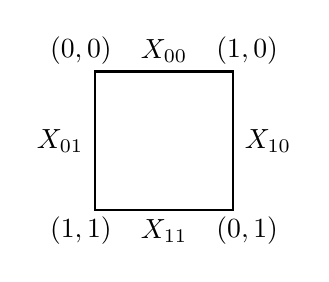
\begin{tikzpicture}[scale=0.88]
        \draw[thick](1,1)--(1,-1)--(-1,-1)--(-1,1)--cycle;

        \draw(-1,1)node{{\Large $\nodeW$}};
        \draw(-1,-1)node{{\Large $\nodeR$}};
        \draw(1,1)node{{\Large $\nodeR$}};
        \draw(1,-1)node{{\Large $\nodeW$}};

        \draw(-1.2,1.3)node{$(0,0)$};
        \draw(1.2,1.3)node{$(1,0)$};
        \draw(-1.2,-1.3)node{$(1,1)$};
        \draw(1.2,-1.3)node{$(0,1)$};

        \draw(0,1.3)node{$X_{00}$};
        \draw(-1.5,0)node{$X_{01}$};
        \draw(1.5,0)node{$X_{10}$};
        \draw(0,-1.3)node{$X_{11}$};
    \end{tikzpicture}
    \caption{The input simplicial model $\cplI$ for $n=2$}
    \label{fig:inputcpl_n2}
\end{figure}



%
%
%
%
%
%

Now we define task solvability, using partial product update. 

\begin{definition}    \label{def:kripkesolvability}
Let $\cplI$ be the input simplicial model and let 
$\actMf{P}$ and $\actMf{T}$ be action models for a protocol and a task, respectively.
A task $\actMf{T}$ is \keywd{solvable} by the protocol $\actMf{P}$ 
if there exists a morphism $\DeltaKrip: \ImProd{\cplI}{\actMf{P}} \to \ImProd{\cplI}{\actMf{T}}$ 
such that %
%
\begin{equation} \label{eq:kripsolve}
    %
    %
    %
    \forall (\preEqClass{p}{X_p},p) \in \ImProd{\cplI}{\actMf{P}}.\: 
    \exists (\preEqClass{t}{X_t}, t)\in\deckrip\bigl((\preEqClass{p}{X_p}, p)\bigr). \:
    \preEqClass{p}{X_p}\subseteq \preEqClass{t}{X_t}.
\end{equation}
%
%
%
%
\end{definition}

%
%
%
%
%
%
%
%
%
%

%
%
%
%
%
%
%


%
Schematically, this definition of solvability can be presented by the following 
diagram-like picture:
\[ \xymatrix{
    \cplI \ar @{} [d] |{\rotatebox{270}{$\subseteq$}} & \ImProd{\cplI}{\actMf{P}} \ar[l]_{\proj_1}\ar[d]^-{\exists \DeltaKrip}\\
    \cplI    & \ImProd{\cplI}{\actMf{T}} \ar[l]^{\proj_1} 
    } \]
where $\proj_1$ is the first projection.     


%
%
%
%
%
%
%

%
%
%
%
Suppose a morphism $\DeltaKrip$ associates
$(\preEqClass{p}{X_p}, p)\in \cplI\{\actMf{P}\}$ with
$(\preEqClass{t}{X_t}, t)\in \cplI\{\actMf{T}\}$. 
Then, in order for this association to be admissible, 
it must respect the inclusion of~\eqref{eq:kripsolve},
%
meaning that,  when $\DeltaKrip$ decides an output $t$ from 
an intermediate output $p$ by the protocol, 
every input contained in 
$\preEqClass{p}{X_p}$, i.e., the set of inputs from which the protocol may produce the output $p$, 
must be an input contained in $\preEqClass{t}{X_t}$, i.e., the set of inputs 
that admit $t$ as the output of the task. 

%
%
%
%

This generalizes the original definition of task solvability given in \cite{Inf:2021:GoubaultLedentRajsbaum},
which makes use of (non-partial) product updates. 
%
The original definition is given by the following commutative diagram, which is obtained by
replacing the models by the product update models, written 
$\cplI[\actMf{P}]$ and $\cplI[\actMf{T}]$, and 
the inclusion in~\eqref{eq:kripsolve} by equality $=$.
\[ \xymatrix{
    & \Prod{\cplI}{\actMf{P}} \ar[dl]_{\proj_1}\ar[d]^-{\exists \delta} \\
    \cplI    & \Prod{\cplI}{\actMf{T}} \ar[l]^{\proj_1} 
    } \]
%
%

%
%
%
%

This definition of the task solvability using product update models is 
equivalent to the topological definition using simplicial complexes \cite{Inf:2021:GoubaultLedentRajsbaum}.  
We can also establish the same equivalence for partial product update models, in the following sense:
Suppose we are given a pair of functions over simplicial complexes 
specifying a task and a protocol. From these specifications we can derive 
the corresponding partial product update models.
Then the task is solvable by the protocol, using partial product update models 
as defined in Definition~\ref{def:kripkesolvability},  
if and only if the task is solvable in the topological sense, i.e., there exists a 
simplicial map that mediates between the complexes of the protocol and the task.

The formal argument for this equivalence is deferred to Appendix~\ref{sec:solvablEq}. 
%
There  we also show that 
the action model $\actMf{A}$ and 
the partial product update model $\ImProd{\cplI}{\actMf{A}}$ 
have isomorphic partial epistemic frames, under a suitable condition. 
%
%
%
%
%


%
%


%
%
%
%
%
%
%
%
%
%
%

%
%
%
%
%
%
%
%
%
%
%
%
%
%

%
%
%
%

%
%
%
%
%
%
%
%
%


 \subsection{Logical obstruction theorem}
 \label{subsec:logicalObstruction}
  
%
%
%
%
%
%
%
%

Combining the above task solvability with the knowledge gain property (Proposition~\ref{prop:knowledgeGainLk}), 
we obtain a proof method for refuting task solvability by a formula of epistemic logic, 
called a \keywd{logical obstruction}~\cite{Inf:2021:GoubaultLedentRajsbaum}.
A logical obstruction $\varphi$ is a guarded positive formula that is valid in the 
partial product update model $\ImProd{\cplI}{\actMf{T}}$ of a task, but not in the
model $\ImProd{\cplI}{\actMf{P}}$ of a protocol. 

\begin{theorem}\label{thm:LOTheorem}
    Let $\ImProd{\cplI}{\actMf{P}}$ and $\ImProd{\cplI}{\actMf{T}}$ be partial product update models
    of a protocol and a task, respectively. 
    If there exists a guarded positive formula $\varphi \in \ModLang_{\Modalfont{K}, \Palive}^{+}$  
    such that $\ImProd{\cplI}{\actMf{T}} \models \varphi$ but $\ImProd{\cplI}{\actMf{P}} \not\models \varphi$, 
    the task is not solvable by the protocol. 
\end{theorem}
\begin{proof}
    Suppose that $\varphi$ is a guarded positive formula such that 
    $\ImProd{\cplI}{\actMf{T}} \models \varphi$ but $\ImProd{\cplI}{\actMf{P}} \not\models \varphi$
    and, by contradiction, that the task is solvable, i.e., there exists 
    a morphism $\delta$ that satisfies the condition~\eqref{eq:kripsolve}. 
    The invalidity for the protocol $\ImProd{\cplI}{\actMf{P}} \not\models \varphi$ 
    means that  $\varphi$ is false for some world $w$ of $\ImProd{\cplI}{\actMf{P}}$.
    Then Proposition~\ref{prop:knowledgeGainLk} implies that there exists a world $w'$ of 
    $\ImProd{\cplI}{\actMf{T}}$ such that $\ImProd{\cplI}{\actMf{T}}, w'\not\models \varphi$. 
    This contradicts to the validity of $\varphi$ in $\ImProd{\cplI}{\actMf{T}}$. 
\end{proof}

%
%
%
%
%

